\section{Epoch models and ancestral range reconstruction}

\subsection{Ancestral range reconstruction}


From the previous section, we created an ancestral state monitor by
\begin{snugshade}
\begin{lstlisting}
mn[3] = mnJointConditionalAncestralState(tree=psi, ctmc=m, filename=out_fn+".states.txt", type="NaturalNumbers", printgen=10, withTips=true, withStartStates=true)
\end{lstlisting}
\end{snugshade}

In this section, we'll use the output from running the DEC analysis assuming all each ordered pair of areas has its own dispersal parameter, and each area has its own extinction parameter.
To generate these results, run
\begin{snugshade}
\begin{lstlisting}
source("RevBayes_scripts/biogeography_DEC_diff.Rev")
\end{lstlisting}
\end{snugshade}


The joint-conditional ancestral state monitor samples the joint distribution of ancestral states every {\tt printgen} iterations over the entire tree, conditioning on the observed tip states.
Due to cladogenesis, the state before speciation and the states inherited after speciation may differ, which we monitor setting {\tt withStartStates=true}.
For convenience we record the tip states using {\tt withTips=true} though these are known through the input data.

The resulting file, {\tt bg\_diff.states.txt}, appears as

\begin{framed}
\begin{lstlisting}
Iteration	start_0	end_0	start_1	end_1	start_2	end_2	start_3	end_3	...
0		2	2	2	4	2	2	2	6	...
10		2	2	4	4	2	2	2	6	...
20		2	2	2	4	2	2	6	6	...
...
\end{lstlisting}
\end{framed}

where columns give the integer-valued range corresponding to either the start or end of a branch leading to a particular node, and each row corresponds to a single sample drawn from the joint distribution of ancestral states.
For example, the lineage leading to the node indexed 1 starts in state 2 (Africa) and ends in state 4 (Eurasia) at iteration 20.
In Section \ref{sec:bayarea}, we will look at how stochastic mappings---the completely realized biogeographic history---may be analysed for data-augmented models.
If you wish to write your own scripts to analyse the ancestral range reconstructions, know that each node's index is recorded when writing a tree's Newick string to file so states may be mapped on to the tree.

\subsection{Data exploration with Phylowood}

To interpret the biogeographical history of primates, we will generate a Phylowood (\url{http://mlandis.github.io/phylowood}) animation.
First, we'll create variables for the relevant files

\begin{snugshade}
\begin{lstlisting}
state_fn = "output/bg_diff.states.txt"
atlas_fn = "data/earth3.still.atlas.txt"
phw_fn = "output/bg_diff.phw.txt"
\end{lstlisting}
\end{snugshade}

then create the animation file

\begin{snugshade}
\begin{lstlisting}
convertToPhylowood(treefile=tree_fn, geofile=atlas_fn, statefile=state_fn, outfile=phw_fn, burnin=0., chartype="NaturalNumbers", bgtype="Range")
\end{lstlisting}
\end{snugshade}

This file summarizes the MCMC output from a RevBayes biogeographical analysis as a Nexus-formatted file, which is used by Phylowood to generate interactive animations to explore biogeographic reconstructions.

\noindent \\ \impmark Open \texttt{http://mlandis.github.io/phylowood}.

\noindent \\ \impmark Drag and drop \texttt{./output/bg\_diff.phw.txt} into the text field.

\begin{figure}[H]
\centering
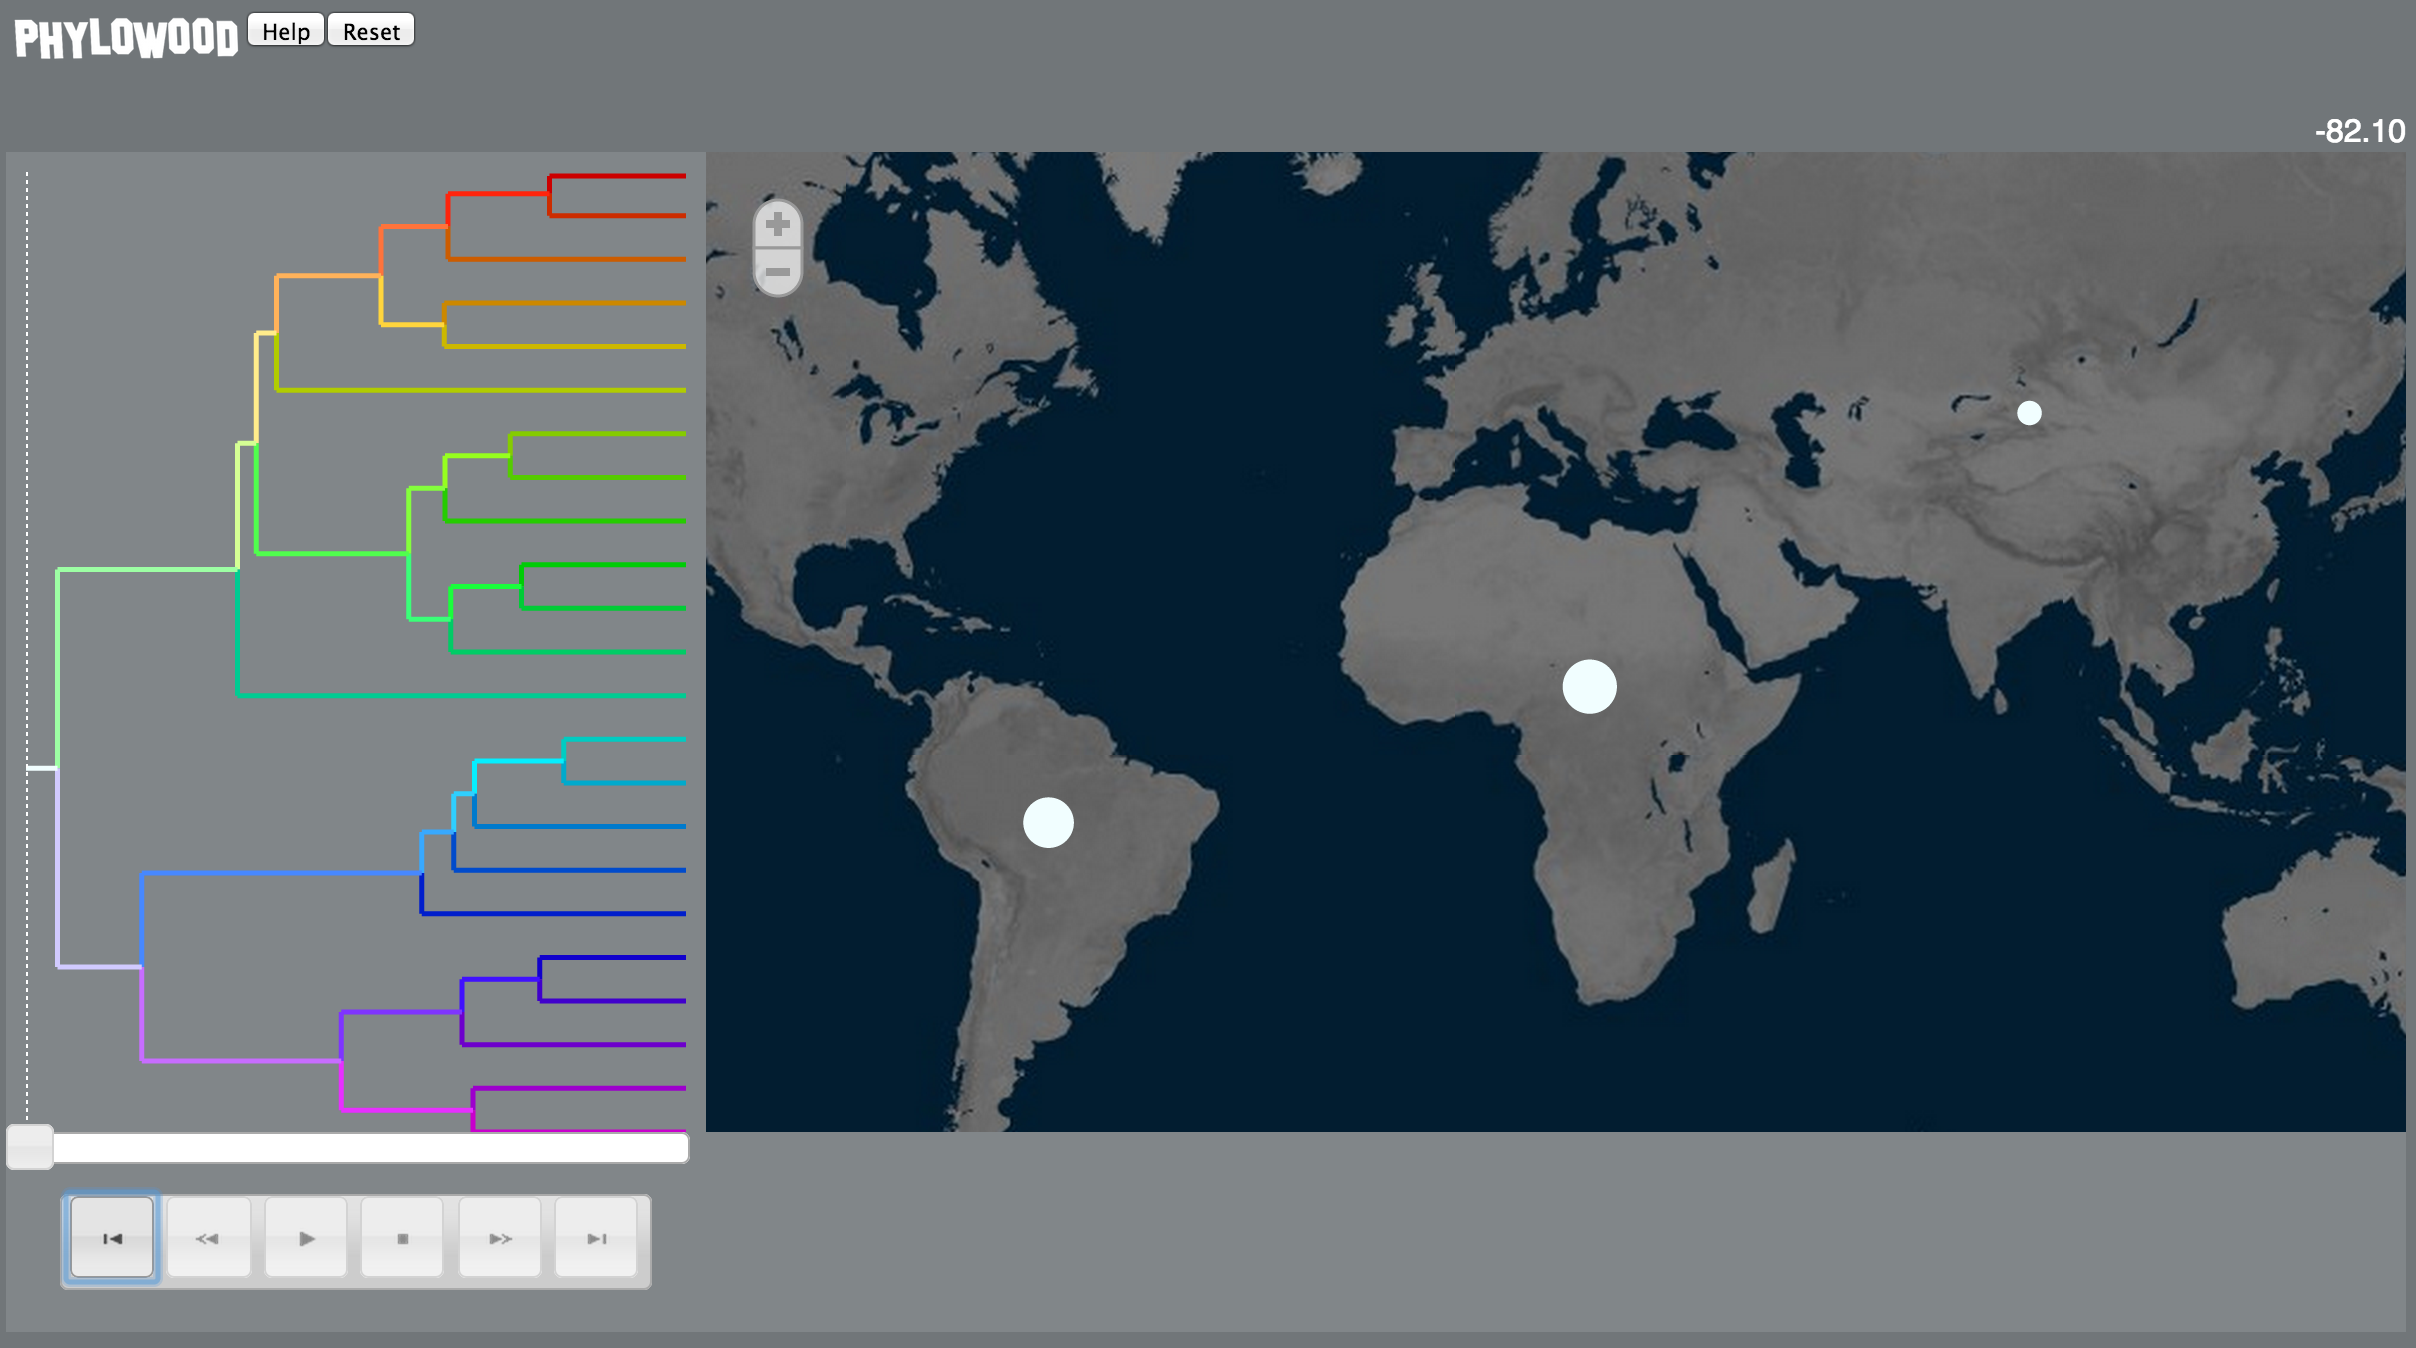
\includegraphics[width=4in]{figures/bg_1_mrca}
\caption{Phylowood frame showing posterior ancestral range of root node.}
\end{figure}

\noindent \\ \impmark Click the Play button to view the animation. \\

There are three control panels to help you filter data: the media panel, the map panel, and the phylogeny panel.
The media buttons correspond to Beginning, Slow/Rewind, Play, Stop, Fast Forward, Ending (from left to right).
The animation will play the timeframe corresponding to the slider.

\noindent \\ \impmark Drag the slider to the right (the present).

\begin{figure}[H]
\centering
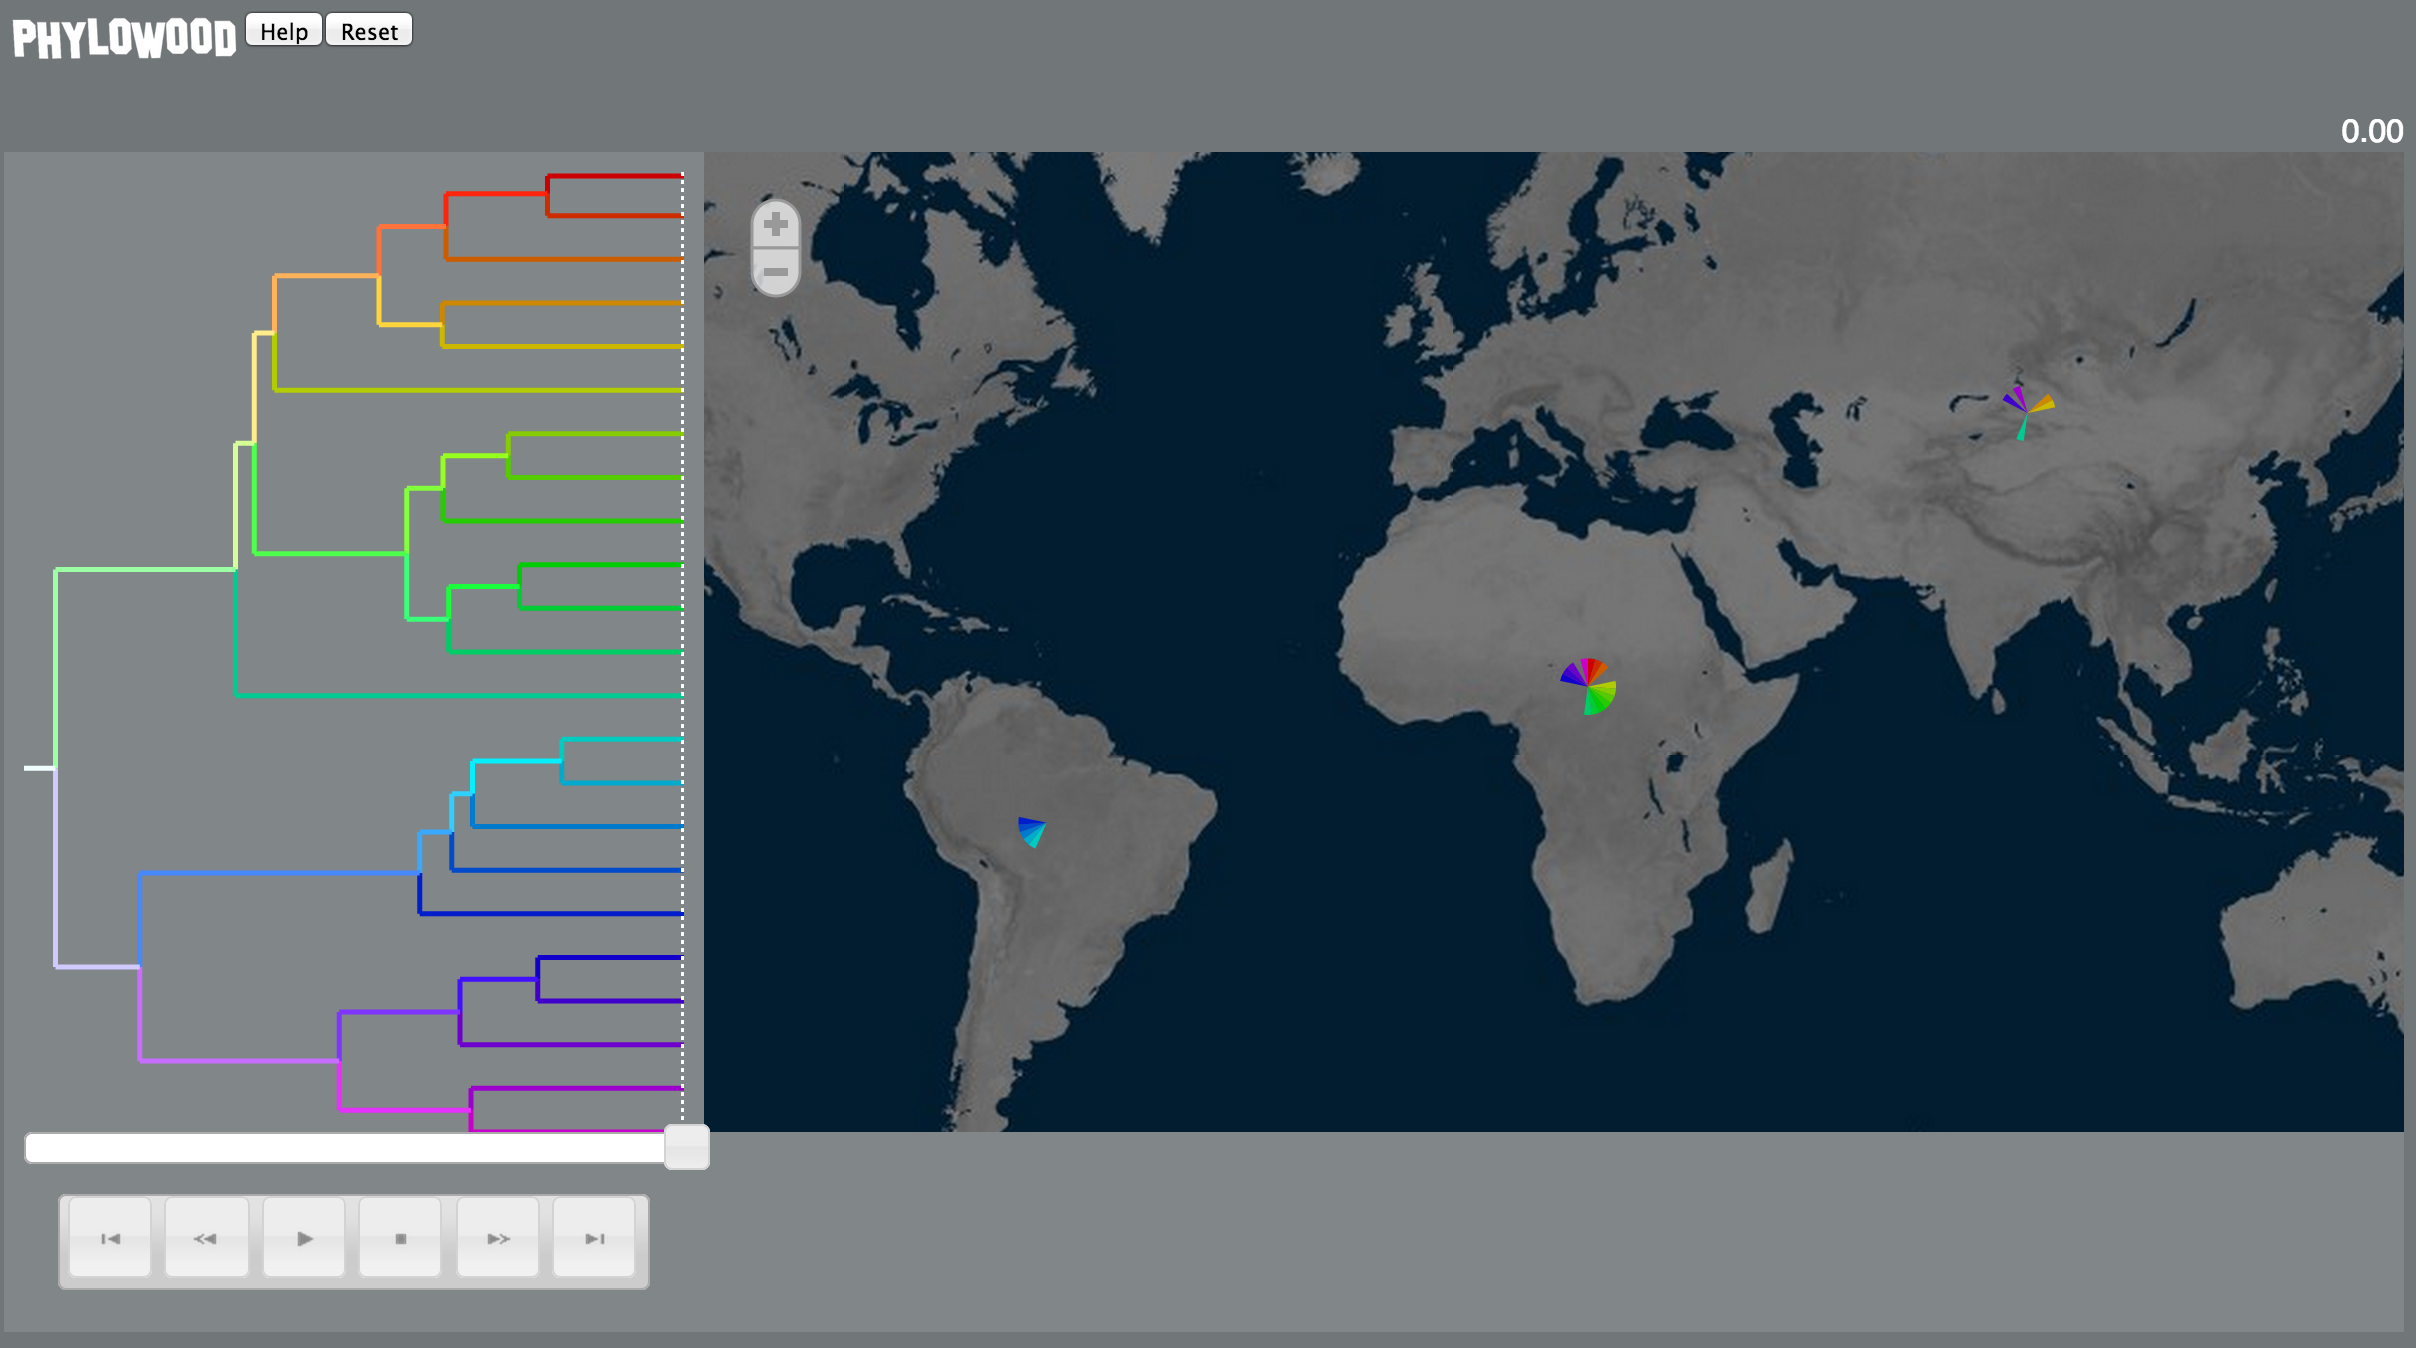
\includegraphics[width=4in]{figures/bg_1_tips}
\caption{Phylowood frame showing distribution of extant taxon ranges.}
\end{figure}

\noindent \\ \impmark Pan and zoom around the map.\\

Marker colors correspond to the phylogenetic lineages in the phylogeny panel.
Markers are split into slices and (loosely) sorted phylogenetically, so nearby slices are generally closely related.
At divergence events, a marker's radius is proportional to the marginal posterior probability the node was present in the area at that time.
Between divergence events, marker's radius is simply an interpolation of the values at the two endpoints.
Some information about geological constraints and cladogenic events is lost.

\noindent \\ \impmark Mouseover an area to learn which lineage it belongs to and its presence probability. \\

Since it's difficult to see how specific clades evolve with so many taxa, Phylowood offers two ways to filter taxa from the animation.
We call the set of a lineage, all its ancestral lineages towards the root, and all descendant lineages a phylogenetic heritage.
The root's heritage is the entire clade.
A leaf node's heritage is a path from the tip to the root.

\noindent \\ \impmark Mouseover a lineage to temporarily highlight the lineage's heritage. Remove the mouseover to remove the highlight effect. \\

The highlight effect is temporary and quickly allows you to single out lineages of interest during animation.
Phylowood also offers a masking effect that persists until an unmask command is issued.

\noindent \\ \impmark Double-click the white root branch to mask the root node's heritage (all lineages). Single click a lineage to unmask that lineage's heritage. \\

\begin{figure}[H]
\centering
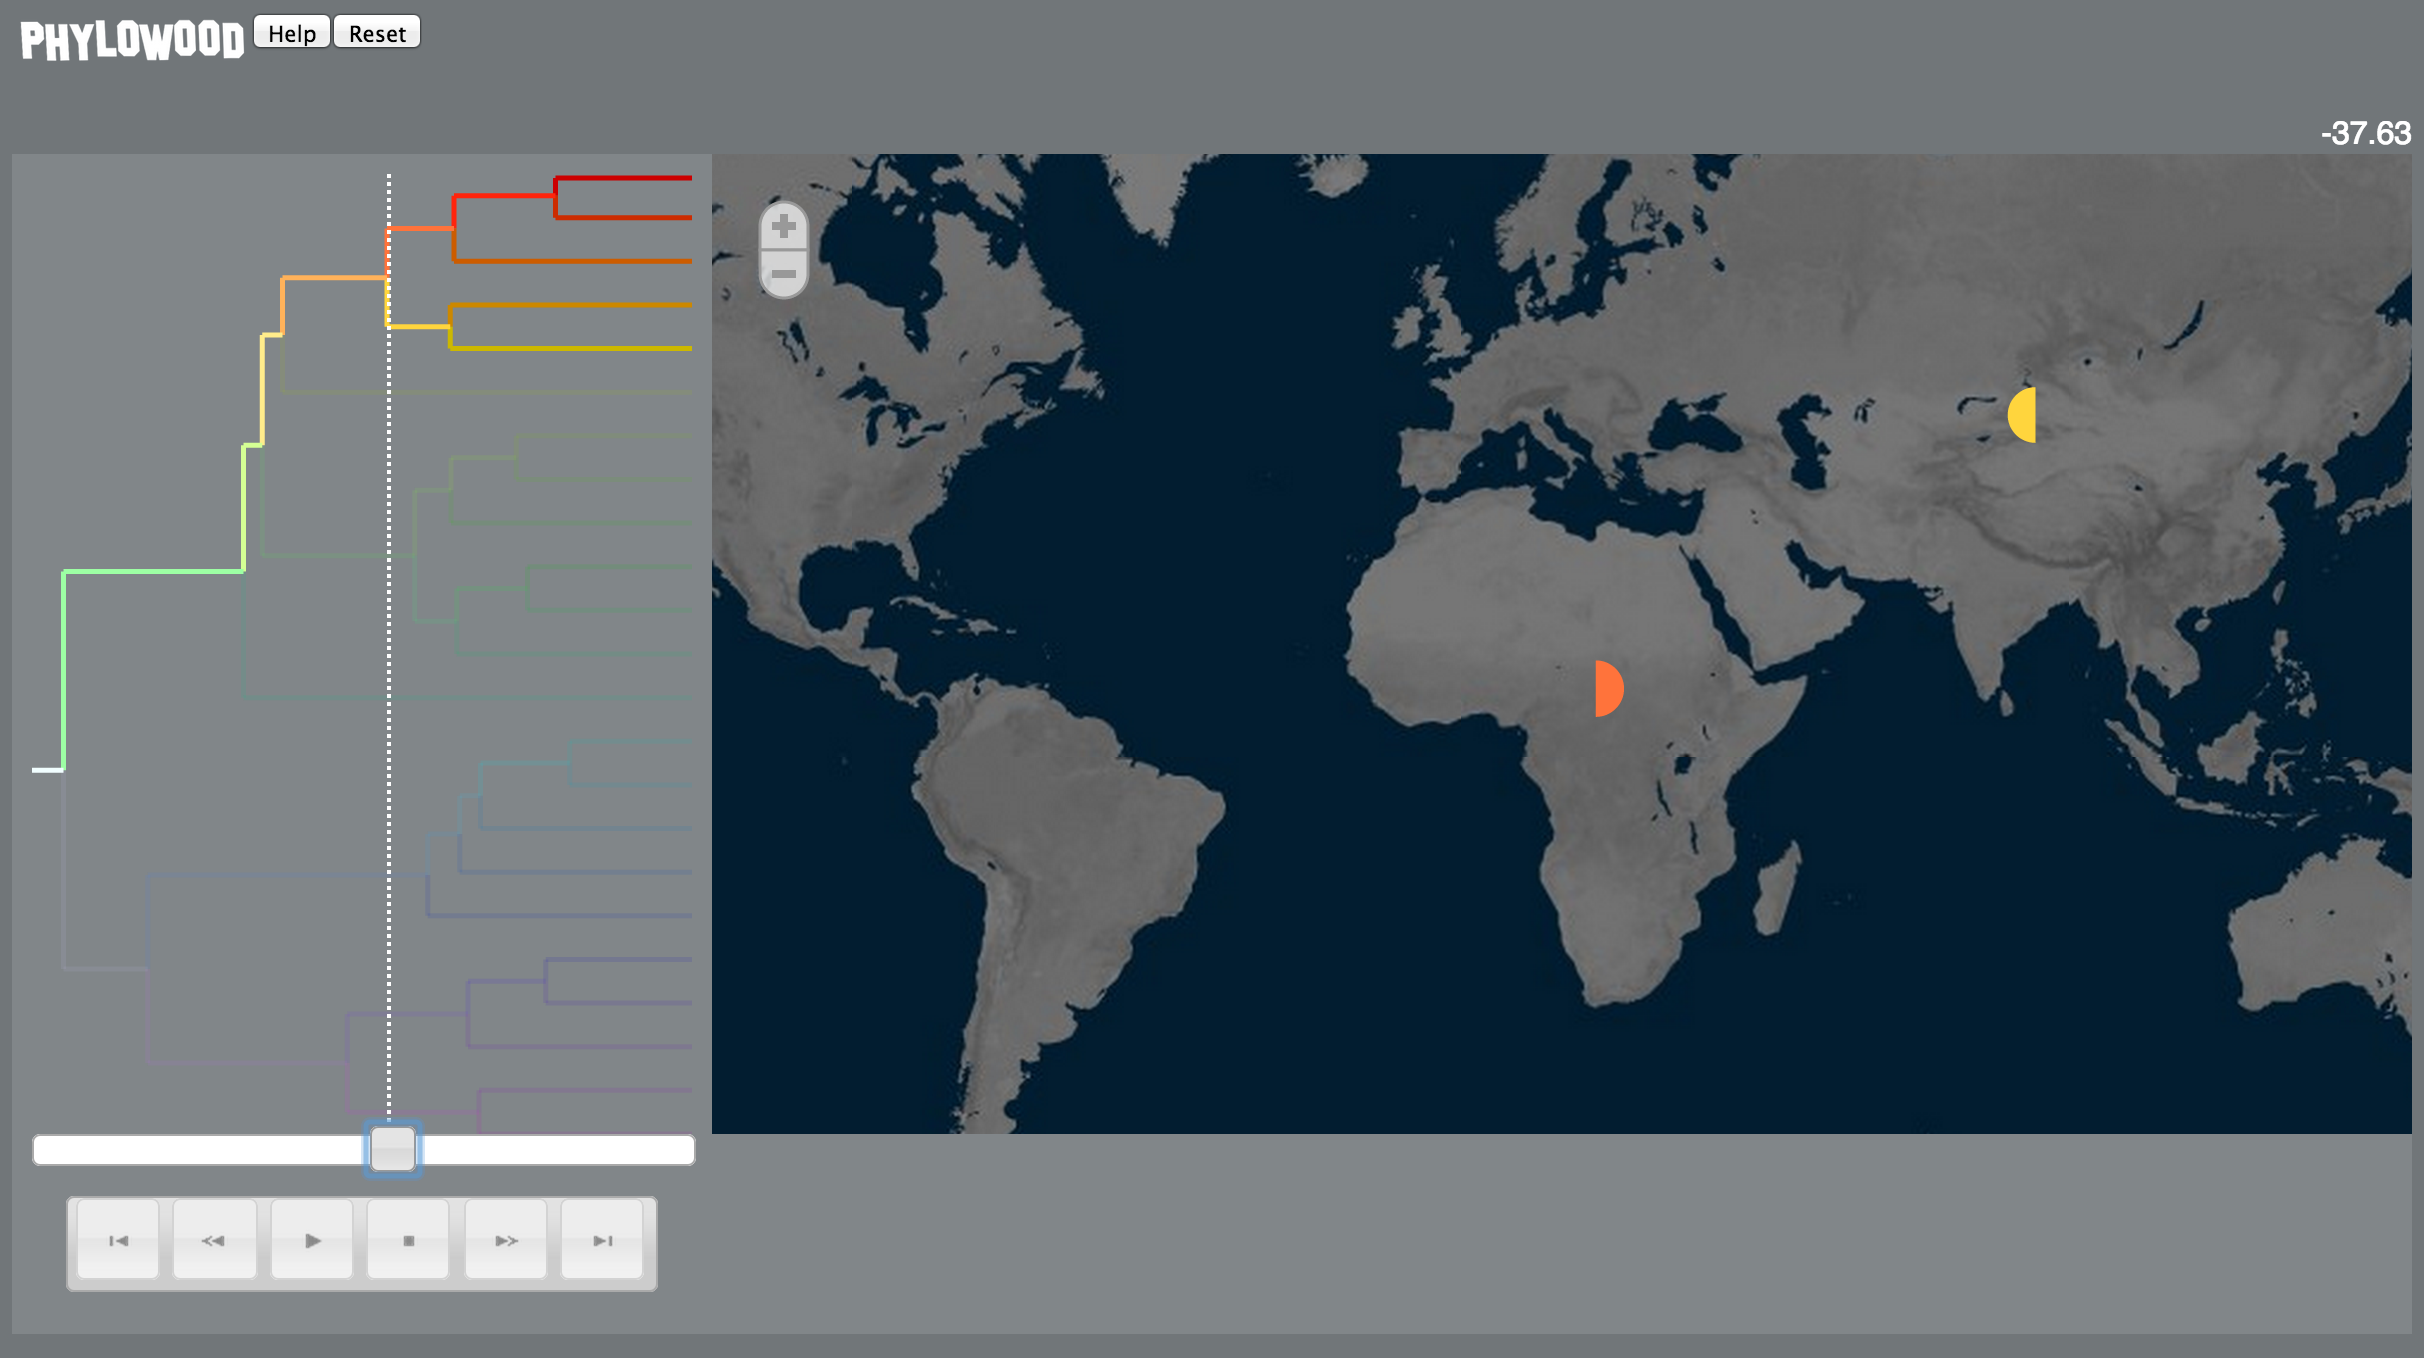
\includegraphics[width=4in]{figures/bg_1_loris}
\caption{Phylowood frame highlighting the ancestral range for the MRCA extant lorises.}
\end{figure}

Now that the masking effects are in place, you're free to interact with other map components.
In addition, the area of marker sizes is only distributed among unmasked lineages.

Visit \texttt{https://github.com/mlandis/phylowood/wiki} to learn more about Phylowood.

Phylowood is useful to understand whether your model generates sensible reconstructions.
Keep in mind the animation and inference both use modern geographies, and that dispersal rates are not modeled to depend on geographical features.
Notice the primate MRCA is widespread in two areas, the New World and Africa.
The root age of the primate tree is about 80Mya, which is about 40Mya after East and West Gondwanaland split to separate modern Africa and South America, so vicariance did not give rise to New World Monkeys.
This is corroborated by examining the fossil record, where the first appearance of primates in South America is about 35Mya.
The standing theory is primates disperse from Africa to South America in a rare ``sweepstakes.''
The naive primate biogeographic model described so far should produce more realistic reconstructions by taking continental drift into account.

\subsection{Epoch models}

To model the effects of geography, we will use {\it epoch} models.
Rather than assuming the evolutionary process is constant with respect to time, it assumes the process is piecewise-constant.
For example, Africa (along with all of Gondwanaland) split from Eurasia (and all of Laurasia) around 180 Mya.
Africa merged with Eurasia only about 50 Mya.
It is reasonable to expect that dispersal rates between Africa and Eurasia were lower before 50 Mya, and higher after 50 Mya until present.

To model this, we will specify one rate matrix that describes anagenic dispersal and extinction processes before for ages $t \geq 50$ and a second rate matrix for the process operating after $0 \leq t < 50$.

To proceed, first we will read in an {\tt Atlas} file, which fully describes the geography per time interval.
For more on the {\tt Atlas} format, see Section XXX.

\begin{snugshade}
\begin{lstlisting}
# read the atlas
atlas <- readAtlas("data/earth3.drift.atlas.txt")
n_epochs = atlas.nEpochs()
times <- atlas.epochTimes()
\end{lstlisting}
\end{snugshade}

This atlas contains two epochs, each with three areas, and a single breakpoint at age 50 (50Mya).
For example, the area for Africa in the second epoch from 50Mya -- present reads
\begin{snugshade}
\begin{lstlisting}
 {
    "latitude": 10.0, 
    "longitude": 20.0,
	"dispersalValues": [ 0.1, 0.0, 1.0 ],
	"extinctionValues": [ 1.0 ],
    "name": "Africa"
}
\end{lstlisting}
\end{snugshade}

The {\tt dispersalValues} values share the ordering of the areas, and each area reports a value regarding it's relationship to other areas.
Here, 0.1 in position 1 indicates the Atlantic Ocean obstructs dispersal from Africa to the Americas, while the 1.0 in position 3 indicates African primates may easily disperse into Eurasia by way of the Arabian Penninsula.
(Note 0.0 in position 2 is the dispersal value from Africa to itself, so the value is arbitrary.)

To extract these values in matrix form

\begin{snugshade}
\begin{lstlisting}
d_prior <- atlas.getValues("dispersal")
\end{lstlisting}
\end{snugshade}

where, for example, the dispersal rate more than 50 Myr in the past (epoch 1) from Africa (area 2) to Eurasia (area 3) is accessed by

\begin{snugshade}
\begin{lstlisting}
d_prior[1][2][3]
\end{lstlisting}
\end{snugshade}

To use these empirical priors to rescale our naive priors

\begin{snugshade}
\begin{lstlisting}
for (t in 1:n_epochs) {
	for (i in 1:n_areas) {
		for (j in 1:n_areas) {
			if (i != j) {
				d_raw[t][i][j] ~ dnExp( 10. )
				mv[mvi++] = mvScale(d_raw[t][i][j], weight=2)
				d[t][i][j] := d_raw[t][i][j] * abs(d_prior[t][i][j])
			} else {
				d[t][i][j] <- abs(0.)
			}
		}
	}
}
\end{lstlisting}
\end{snugshade}

We'll make no strong prior assumptions about epochs or areas differentially affecting extinction rates.

\begin{snugshade}
\begin{lstlisting}
# set up extinction per epoch
e_prior <- atlas.getValues("extinction")
for (t in 1:n_epochs) {
	for (i in 1:n_areas) {
		e_raw[t][i] ~ dnExp( 10. )
		mv[mvi++] = mvScale(e_raw[t][i], weight=2)
		e[t][i] := e_raw[t][i] * abs(d_prior[t][i][1])
	}
}
\end{lstlisting}
\end{snugshade}

Now we have dispersal rates and extinction rates per epoch in the matrices {\tt d} and {\tt e}.

Extant primate ranges do not appear capable of spanning all three areas simultaneously, so we might constrain the range evolution process to only allow ranges of size two

\begin{snugshade}
\begin{lstlisting}
rangeSize <- simplex(0,1,1,0)
\end{lstlisting}
\end{snugshade}

where the first and last elements are set to zero, so ranges cannot be size 0 or size 3.
By calling {\tt fnDECRoot} with the {\tt rangeSize} parameter, we can also force the MRCA range size to be a single area.

\begin{snugshade}
\begin{lstlisting}
rf := fnDECRoot( rep(1,n_states), rangeSize=simplex(0,1,0,0) )
\end{lstlisting}
\end{snugshade}

Next, we'll create a rate matrix for each epoch

\begin{snugshade}
\begin{lstlisting}
for (t in 1:n_epochs) {
	rates[t] ~ dnGamma(2,2)
	mv[mvi++] = mvScale(rates[t], weight=2)	
	q[t] := fnDECRateMatrix(d[t], e[t], rangeSize)
}
\end{lstlisting}
\end{snugshade}

with {\tt rates} being an epochal rate multiplier, each with mean 1.
Notice, we construct {\tt q[t]} for each epoch {\tt t} in {\tt num\_epochs}, using the epoch's dispersal values {\tt d[t]} and extinction values {\tt e[t]}.
Finally, we wrap our vector of rate matrices, {\tt q}, along with the epoch boundary times, {\tt times}, and  our epochal rates, {\tt rates} 

\begin{snugshade}
\begin{lstlisting}
q_epoch := fnEpoch( Q=q, times=times, rates=rates )
\end{lstlisting}
\end{snugshade}

Parameters like {\tt clado\_prob} and {\tt clock\_bg} still need to be created, as they were in the previous section.

Otherwise, the model is created as before, except passing {\tt q\_epoch} into {\tt dnPhyloCTMCClado}.

\begin{snugshade}
\begin{lstlisting}
m ~ dnPhyloCTMCClado( tree=psi, Q=q_epoch, rootFrequencies=rf, cladoProbs=clado_prob, branchRates=clock_bg, nSites=1, type="NaturalNumbers" )
m.clamp(data)
mdl = model(m)
\end{lstlisting}
\end{snugshade}

This biologically and geographically informed model produces a more realistic range reconstruction

\begin{figure}[H]
\centering
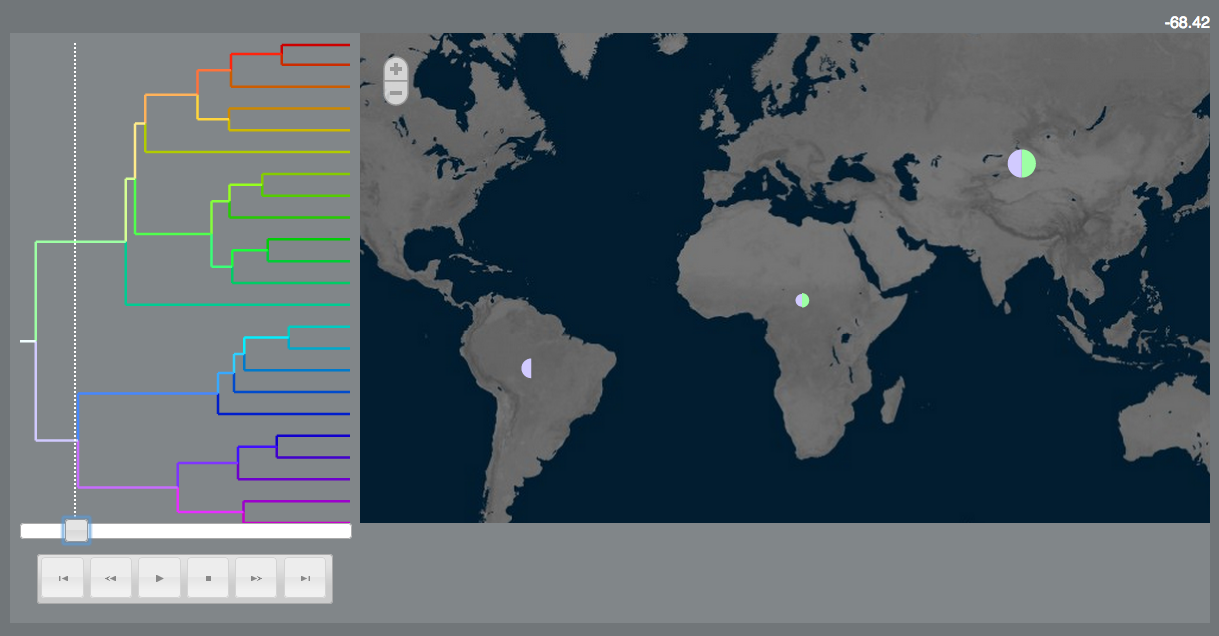
\includegraphics[width=4in]{figures/bg_2_epoch}
\caption{Phylowood frame showing Asian origin of primates, with subsequent dispersal into Africa and Americas.}
\end{figure}


This example model may be run by typing

\begin{snugshade}
\begin{lstlisting}
RevBayes_scripts/biogeography_epoch.Rev}
\end{lstlisting}
\end{snugshade}

which also produces the above Phylowood animation file.
